 \documentclass[12pt]{article}
\usepackage[a4paper, margin=.30in]{geometry}

\usepackage{array}
\usepackage{graphicx, subfig, wrapfig, fancyhdr, lastpage }
\newcommand\headerMe[2]{\noindent{}#1\hfill#2}
\usepackage[mathscr]{euscript}



\pagestyle{fancy}
\fancyhf{}

\rfoot{\em{Page \thepage \hspace{1pt} / \pageref{LastPage}}}
\begin{document}

\headerMe{Royaume du Maroc}{année scolaire \emph{2021-2022}}\\
\headerMe{Ministère de l'Éducation nationale, }{  Professeur :\emph{Zakaria Haouzan}}\\
\headerMe{du Préscolaire et des Sports}{Établissement : \emph{Lycée SKHOR qualifiant}}\\

\begin{center}
Devoir  N°1 \\
   Filière Tronc Commun Scientifique\\
Durée 1h30
\\
    \vspace{.2cm}
\hrulefill
\Large{Chimie 7pts}
\hrulefill\\

    %\emph{Les Trois parties sont indépendantes}
\end{center}
%end Headerss------------------------
 \section*{Partie 1 :Classification périodique des éléments chimiques \dotfill (7pts) }
Un élément X se trouve dans la 3 ème période et dans le groupe (II) du tableau périodique simplifiée.
\begin{enumerate}
    \item Déterminer la structure électronique de l'atome de l'élément X.\dotfill(1pt)

    \item Déterminer le numéro atomique de cet élément ainsi que son symbole et son nom. \dotfill(1pt)
    \item Nommer la famille à laquelle cet élément chimique appartient.\dotfill(1pts)
    \item Citer un autre éléments appartenant à la même famille.\dotfill(1pt)
 \item Quel ion monoatomique est susceptible de se former à partir de l’atome cet élément ?\dotfill(1pt)
 \item Quel est le nombre d'électrons de valence que possède l’atome X ?\dotfill(1pt)
 \item Quel est le nombre totale d'électrons que possède l’atome X?\dotfill(1pt)
\end{enumerate}
%__________________Chimie ______________________-
%%%%%%%+_+_+_+_+_+_+_+_+_Partie1

%_____________________________________PHYSIque Partie 22222____________________________________________________________________________
\begin{center}
    %\vspace{2cm}
\hrulefill
\Large{Physique 13pts}
\hrulefill\\
    \emph{Les deux parties sont indépendantes}
\end{center}
%end Headerss------------------------

 \section*{Partie 1 :Équilibre d’un corps solide soumis à trois forces non parallèles (7 pts)}

\begin{wrapfigure}[5]{r}{0.36\textwidth}
    \vspace{-1.8cm}
    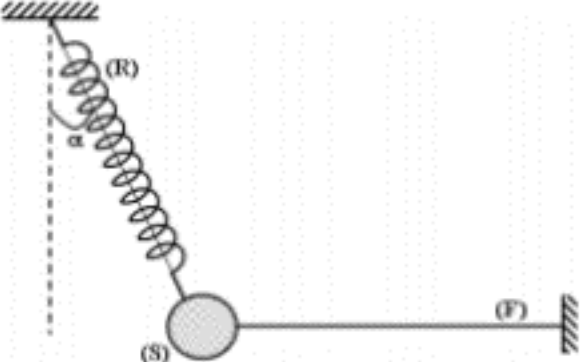
\includegraphics[width=0.36\textwidth]{./img/pendule_simple.png}
\end{wrapfigure}

On considère un solide (S) de masse
m=200g, accroché à un ressort (R) et à un fil (F) d'intensité F = 1.2N comme l’indique la figure ci-contre.

Le ressort de raideur K=40N/m est
incliné d’un angle $\alpha$=30° par rapport à la
verticale. Le fil est horizontal. On prendra g=10N/Kg.

\begin{enumerate}
    \item Faire le bilan des forces qui
s’exercent sur le solide (S) et les
        représenter sur la figure.\dotfill(1pt)

    \item Ecrire la condition de l’équilibre du solide (S).\dotfill(1pt)
    \item Donner les expressions des coordonnées de chacune des forces dans le repére $(O, x, y)$ en fonction de leurs intensités.\dotfill(1pts)
    \item Déterminer la tension T du ressort : \dotfill(2pt)
        \begin{enumerate}
            \item Par méthode analytique.
            \item Par méthode géométrique en utilisant une échelle convenable
        \end{enumerate}
    \item déduire l’allongement du ressort.\dotfill(1pt)
    \item déterminer la longueur finale L du ressort à l’équilibre sachant que sa longueur initiale est L0 = 20 cm \dotfill(1pt)
\end{enumerate}

\vspace{3cm}

\hrulefill\\
%_________________partie 2  : gravitation universelle :)
\section*{Partie 2 : Équilibre d'un corps solide en rotation autour d'un axe fixe\dotfill(6pts)}
Un homme maintient en équilibre un panneau de centre G, de
masse $m = 50kg$, et de longueur $OA = 2m$ dans une position
inclinée d’un angle $\alpha$ = 60° avec le sol. Il exerce en H, à la
distance $OH = 1,7m$ une force $\vec{F}$ perpendiculaire au panneau
comme indique la figure ci-contre. Le panneau peut tourner
autour de l’axe $(\Delta)$ passant par O

\begin{center}

    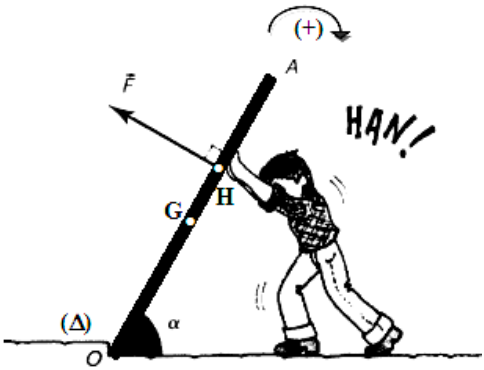
\includegraphics[width=0.36\textwidth]{./img/rotation.png}
\end{center}
\begin{enumerate}
    \item Faire l’inventaire des forces appliquées sur le panneau, et les
        représenter sur la figure.\dotfill(2pts)
    \item Enoncer le théorème des moments. \dotfill(1pt)
\item Trouver l’expression du moment de chaque force appliquée
    sur le panneau \dotfill(1pt)
\item En utilisant le théorème des moments, montrer que l’expression de l’intensité de la force $\vec{F}$ appliquée par l’homme s'écrit sous la forme :$$F = \frac{m.g.OA.cos\alpha}{2.OH}$$
    , et calculer sa valeur. \dotfill(2pts)
        \end{enumerate}

\end{document}
